\documentclass{article}
\usepackage[utf8]{inputenc}
\usepackage[spanish]{babel}
\usepackage{enumerate} % enumerados
\usepackage{graphicx}
\usepackage{hyperref}
\usepackage{minted}

\title{Práctica N° 13 - FdLP}
\author{Christian Omar Rodriguez Huamanñahui\\
crodriguezh@ulasalle.edu.pe}
\date{OCT 2022}

\maketitle
\clearpage
\usepackage[margin=0.5in]{geometry}
\begin{document}
\documentclass

\tableofcontents
\clearpage
\section{Ejercicio 1}
Investigue el concepto de first class en Javascript y muestre una pequeña definición seguida ejemplos. (2 puntos)\\
\\La función se considera de "Firts Class" o "Primera Clase" si es apto para almacenar en una variable, también se pueden asignar funciones a variables, pasar funciones como parámetros hacia otras funciones o retornar funciones desde otra función. Eso es lo que define una función de primera clase.\\
\\
Ejemplo:
\begin{minted}{javascript}
//Hola Mundo: Firts Class en JavaScript
function decirHolaMundo() {
    return () => {
    console.log("¡Hola Mundo!");
    };
} 

//Suma: Firts Class en JavaScript
function suma(x,y) {  
    return x + y;  
}  
let sum = suma;

//Resta: Firts Class en JavaScript
function resta(x,y) {  
    return x - y;  
}  
let rest = resta;


console.log(decirHolaMundo())
//OUT: FUNCIÓN "DecirHolaMundo"
console.log(suma(30,12))
//OUT: 42
console.log(resta(30,12))
//OUT: 18
\end{minted}

\begin{figure}[h]
\centering
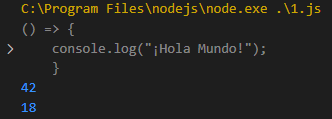
\includegraphics[scale=1.5]{EJERCICIO1.png}
\end{figure}



\newpage
\section{Ejercicio 2}
Describa la diferencia entre Currying and Partial Application. Incluya ejemplos. (2 puntos)

En otras palabras, "currying" y "aplicación parcial" son dos funciones totalmente diferentes. Currying toma exactamente 1 entrada, mientras que la aplicación parcial toma 2 (o más) entradas.
\\
\\
- Ejemplo en Currying: RESTA
\begin{minted}{javascript}
//Ejemplo en Currying: RESTA
let restaCurrying = (a) =>{
    return (b) =>{
        return a - b;
    }
}
console.log(restaCurrying())
//OUT: Currying de RESTA
\end{minted}
\\
- Ejemplo en Partial Aplication: RESTA

\begin{minted}{javascript}
//Ejemplo en Partial Aplication: RESTA
function restaPartial(a, b) {  
    return a - b;  
}  
let rest = restaPartial; 
console.log(restaPartial(30,12))
//OUT: 18
\end{minted}

\begin{figure}[h]
\centering
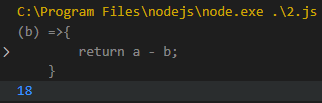
\includegraphics[scale=1.5]{EJERCICIO2.png}
\end{figure}



\newpage
\section{Ejercicio 3}
Implemente una función que calcule el volumen de un cilindro. Incluya la versíon normal y una aplicando Currying. (2 puntos)
\\
- Ejemplo con CURRYING: VOL. CILINDRO (30,12)
\begin{minted}{javascript}
//VOL. CILINDRO: CURRYING
let volumenDelCilindro = (r,h) => r*r*h*Math.PI;
console.log(volumenDelCilindro(30,12))
//OUT: 33929.20065876977
\end{minted}
\\
- Ejemplo con IMPLEMENTACIÓN "NORMAL": VOL. CILINDRO (12,30)
\begin{minted}{javascript}
//VOL. CILINDRO: "NORMAL"
let VolumenDelCilindroCurrying = (r) =>{
    return (h) =>{
        return r*r*h*Math.PI
    }
}
console.log(VolumenDelCilindroCurrying(12)(30))
//OUT: 13571.680263507906

\end{minted}

\begin{figure}[h]
\centering
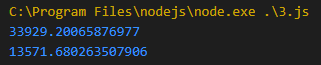
\includegraphics[scale=1.5]{EJERCICIO3.png}
\end{figure}


\newpage
\section{Ejercicio 4}
Cree una funciòn joinWords que una varios parametros de tipo string. (3 puntos)


\begin{minted}{javascript}
//Cree una funcion joinWords que una varios parametros de tipo string.
function joinWords(...args){
    //En el siguiente fragmento se determina lo que se busca añadir entre strings 
    //En este caso lo dejamos vacío, debido a que el propio input inserta los espacios: " "
    const result = args.join('');
    const UnirPalabras = (...innerargs)=>{
        if(innerargs.length===0) return result;
        return joinWords(...args, innerargs)
    }
    return UnirPalabras;
}
//AVISO: LOS PRINT FINALIZAN UNA VEZ ENCUENTREN EL VACÍO: ()
result = joinWords ('Hello ') () ;
console .log ( result ); 
//OUT: Hello
result = joinWords ('There ')('is ')('no ')('spoon.') () ;
console .log ( result );
//OUT: There is no spoon.
\end{minted}
\begin{figure}[h]
\centering
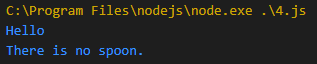
\includegraphics[scale=1.5]{EJERCICIO4.png}
\end{figure}



\newpage
\section{Ejercicio 5}
Implemente una funciòn delayInvoc que en cada invocaciòn incremente la variable total con el valor enviado como parámetro. (3 puntos)

\begin{minted}{javascript}
var total = 0;
var delayInvoc = function (a) {
// your code here
};
delayInvoc (4) (5)
console .log ( total ); //9
delayInvoc (4) (5) (8)
console .log ( total ); // 26
\end{minted}

\begin{minted}{javascript}
//Implemente una función delayInvoc que en cada invocacion incremente la variable total con el
//valor enviado como parametro.
let total = 0;
//FUNCIÓN: Sumar valores y pasar al siguiente valor hasta llegar al vacío
function delayInvoc(...args) {
    let result= args.reduce((r,v)=> r+v);

    const sum = (...innerargs)=>{
        if (innerargs.length === 0) return result;
        return delayInvoc(...args, ...innerargs)
    }
    return sum;
};
//AVISO: LOS PRINT FINALIZAN UNA VEZ ENCUENTREN EL VACÍO: ()
let total1 = delayInvoc(4)(5)();
console.log (total1); //9
//OUT de 4+5: 9
total1 = delayInvoc(4)(5)(8)();
console.log (total1);
//OUT de 4+5+8: 17
\end{minted}
\begin{figure}[h]
\centering
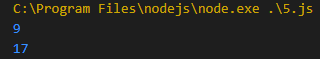
\includegraphics[scale=1.5]{EJERCICIO5.png}
\end{figure}



\newpage
\section{Ejercicio 6}
Implemente una función curry que tome como argumento cualquier función f y retorne la versión curried de f. (4 puntos)

\begin{minted}{javascript}
function abc (a, b, c){
return a+b+c;
}
function curry (f) {
// your code here
}
var curriedAbc = curry ( abc );
console .log ( curriedAbc (2) (3) (4) ); // 9
console .log ( curriedAbc (2 ,3) (4) ); // 9
console .log ( curriedAbc (2) (3 ,4) ); // 9
console .log ( curriedAbc (2 ,3 ,4) ) ; // 9
\end{minted}

\begin{minted}{javascript}
//Implemente una función curry que tome como argumento cualquier función f y retorne la versión curried de f.
//FUNCIÓN: Sumar c/u de los 3 parámetros 
function abc(a, b, c) {
return a + b + c;
}
function curry (f) {
    return suma = (...args) => {
        if (f.length !== args.length) return suma.bind(null, ...args);
    return f(...args);
    };
}
var curriedAbc = curry(abc);
console.log(curriedAbc(2)(3)(4));
//OUT: 9
console.log(curriedAbc(2, 3)(4));
//OUT: 9 
console.log(curriedAbc(2)(3, 4));
//OUT: 9
console.log(curriedAbc(2, 3, 4));
//OUT: 9
\end{minted}
\begin{figure}[h]
\centering
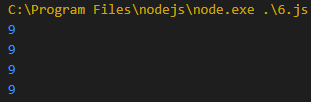
\includegraphics[scale=1.5]{EJERCICIO6.png}
\end{figure}



\end{document}
